\documentclass{beamer}
%\setbeamersize{text margin left=10pt,text margin right=10pt}
\usetheme{metropolis}
\usepackage{listings}
\usepackage{amsfonts}
\usepackage{dsfont}
\usepackage{amsmath}
\usepackage{bbm}
\usepackage{verbatim}
%\usepackage{tipa}
\usepackage{tikz}
\usetikzlibrary{fit}
\usepackage{color}
\usepackage{booktabs}
\usepackage{tipa}
\usepackage{amssymb}
\usepackage{verbatim}
\usepackage[absolute,overlay]{textpos}
\usepackage{pifont}% http://ctan.org/pkg/pifont
\usepackage{caption}
\usepackage{subcaption}
\newcommand{\cmark}{\ding{51}}%
\newcommand{\xmark}{\ding{55}}%
\usetikzlibrary{bayesnet}
\usetikzlibrary{decorations.markings}
\usetikzlibrary{decorations.pathmorphing}
\tikzset{squiggle/.style={decorate, decoration={snake,amplitude=.4mm}}}
\usepackage{xcolor}
\definecolor{pop1}{HTML}{1F78b4}
\definecolor{pop2}{HTML}{164C13}
\definecolor{pop3}{HTML}{d95F02}
\definecolor{orange}{HTML}{d95F02}
\definecolor{teal}{HTML}{1b9e77}
\newcommand{\pop}[1]{\textcolor{pop1}{#1}}
\newcommand{\popp}[1]{\textcolor{pop2}{#1}}
\newcommand{\tree}[1]{\textcolor{pop3}{#1}}
\newcommand{\orange}[1]{\textcolor{orange}{#1}}
\newcommand{\teal}[1]{\textcolor{teal}{#1}}
\newcommand{\code}[1]{{\footnotesize\texttt{#1}}}
\newcommand{\greenCode}[1]{{\footnotesize\popp{\code{#1}}}}
\newcommand{\blueCode}[1]{{\footnotesize\pop{\code{#1}}}}
\definecolor{backgroundGreen}{HTML}{23373b}
\lstset{escapeinside={<@}{@>}}
\usepackage{pgf}  

%% \usepackage[sfdefault]{FiraSans} %% option 'sfdefault' activates Fira Sans as the default text font
%% \usepackage[T1]{fontenc}
%% \renewcommand*\oldstylenums[1]{{\firaoldstyle #1}}


\newcommand{\Expect}{\mathds{E}} %{{\rm I\kern-.3em E}}
\newcommand{\indicator}{\mathds{1}} %{{\rm I\kern-.3em E}}
\newcommand{\expect}{\mathds{E}} %{{\rm I\kern-.3em E}}
\newcommand{\probability}{\mathds{P}} %{{\rm I\kern-.3em P}}
\DeclareMathOperator*{\argmin}{arg\,min} % thin space, limits underneath in displays
\DeclareMathOperator*{\argmax}{arg\,max} % thin space, limits underneath in displays

\usepackage[absolute,overlay]{textpos}

\newcommand{\nextForm}[1]{\rotatebox[origin=c]{270}{$_{\curvearrowright}$}$_{#1}$}
 
\usepackage{amsfonts}
\usepackage{tabularx}
%\usepackage{color}
\usepackage{graphicx}
\usepackage{booktabs}
\usepackage{xcolor}
\usepackage{tikz}
\usetikzlibrary{trees}
\usetikzlibrary{fit}
\usetikzlibrary{calc}
\usetikzlibrary{bayesnet}
\usepackage[absolute,overlay]{textpos}
\usepackage{stmaryrd}
\newcommand{\sem}[1]{\llbracket #1\rrbracket}
\newcommand{\tuple}[1]{\ensuremath{\left \langle #1\right \rangle}}
\newcommand{\messageOverlay}[1]{
      \tikz[overlay,remember picture]
      \node[align=left,fill=backgroundGreen,text=white] at (current page.center){#1};
}
\usepackage{booktabs}
\usepackage{tipa}
\usepackage{amssymb}
\usepackage{verbatim}
\usepackage[absolute,overlay]{textpos}
\usepackage{pifont}% http://ctan.org/pkg/pifont
\newcommand{\cmark}{\ding{51}}%
\newcommand{\xmark}{\ding{55}}%
\usetikzlibrary{bayesnet}
\usetikzlibrary{decorations.markings}

\newcommand\Wider[2][3em]{%
\makebox[\linewidth][c]{%
  \begin{minipage}{\dimexpr\textwidth+#1\relax}
  \raggedright#2
  \end{minipage}%
  }%
}

\newcommand{\denotation}[1]{{\llbracket #1 \rrbracket}}

\usepackage[utf8]{inputenc}
\newcommand{\reduce}{\longrightarrow}
\usepackage{amssymb}% http://ctan.org/pkg/amssymb
\usepackage{pifont}% http://ctan.org/pkg/pifont

\usepackage{fancyvrb}

\usepackage[most]{tcolorbox}
\definecolor{block-gray}{gray}{0.10}
\newtcolorbox{mycode}{colback=block-gray,grow to right by=0mm,grow to left
by=0mm, boxrule=0pt,boxsep=0pt,breakable,fontupper=\color{white}}

%% Program ::=
%%   (if Bool List
%%     (append RecursiveList
%%             RecursiveList
%%             RecursiveList))
%% RecursiveList ::= List
%%          | (recurse List)

            

\usepackage{arydshln}

\newcommand{\Expect}{\mathds{E}} %{{\rm I\kern-.3em E}}
\newcommand{\Probability}{\mathds{P}} %{{\rm I\kern-.3em P}}

\DeclareMathOperator*{\argmax}{arg\,max}
%Information to be included in the title page:
\title{GPS / Program Induction}%,\\ by learning to write code that writes code}
%% \author{Kevin Ellis}
%% \institute{MIT} 
%% \date{2020}
  
 
\begin{document}
 
\frame{\titlepage}




\begin{frame}{Human program induction everywhere}
\begin{tikzpicture}
  \node(Lisp) at (0,0) {\includegraphics[width = 5cm]{ecFigures/1975.png}};
  \visible<2->{
    \node(colorless) at (6,0) {\includegraphics[width = 5cm]{ecFigures/colorless.png}};
    \node at ([yshift=-2cm]colorless.south) {\includegraphics[width = 4cm]{ecFigures/child.jpg}};
  }
  \visible<3->{
    \node(aqueduct) at ([yshift=-1cm,xshift=0cm]Lisp.south) {\includegraphics[width = 5cm]{ecFigures/aqueduct.jpg}};
    \node(arch) at ([xshift=1cm,yshift=0cm]aqueduct.south) {\includegraphics[width = 1.5cm]{ecFigures/arch.jpg}};
  }
  \visible<4->{
    \node at ([yshift=-1cm,xshift=-2cm]aqueduct.south) {\includegraphics[width = 2cm]{ecFigures/tapestry.jpg}};
    \node(wiringDiagram) at ([yshift=-1cm,xshift=1.6cm]aqueduct.south) {\includegraphics[width = 5cm]{ecFigures/wiringDiagram.jpg}};
  }
  %% \visible<5->{
  %%   \node at ([xshift=2cm,yshift=1cm]wiringDiagram.east) {\includegraphics[width = 5cm]{tree.jpg}};
  %%   }
  \end{tikzpicture}

\end{frame}

%% \begin{frame}{Engineering the language of thought}
%%  \begin{tikzpicture}
%%     \node () {\includegraphics[width = 15.6cm]{theory.png}};
%%     \node at (-5,-4) {  Ullman et al 2012};
%%     \end{tikzpicture}
%% \end{frame}

\begin{frame}{Human program induction everywhere}
  \begin{tikzpicture}
    \node at(0,0) {\includegraphics[width = 8cm]{../ecPaper/characters.png}};
    \node at(-3,2) {\includegraphics[width = 8cm]{../ecPaper/Brendan.jpg}};

    \node at (-5,-4) {  Lake et al 2015};
    \end{tikzpicture}
\end{frame}


\begin{frame}{Exploration-Compression}
  Dechter et al. 2013

  What if we don't have the right programming language for solving our problems?

  \pause
  
  Idea: Iteratively grow the language, alternating problem-solving and language-growing. Grow the language by ``compressing out'' reused program components, and cache those components in a learned library

\end{frame}

\begin{frame}[t]{Exploration-Compression as Bayesian inference}
  %  \includegraphics[width = 11cm]{ecFigures/animation/EC.eps}
\centering  \begin{tikzpicture}[scale=1,line width=0.5mm]

  \node[latent,scale=1] at (3.5,3) (dx){Lib};
  \node[latent,scale=1] at ([yshift=-1.5cm]dx) (zp){prog};
  \node[obs,scale=1] at ([yshift=-1.5cm]zp) (xp) {data};
  \node[latent,scale=1] at ([xshift=2cm]zp) (zp1){prog};
  \node[obs,scale=1] at ([xshift=2cm]xp) (xp1) {data};
  \draw [->] (zp1.south) -- (xp1.north);
  \draw [->] (dx.south) -- (zp1.north);
  %\draw [->,red] (xp1.east) to[out = 30,in = -30] node(nn){} (zp1.east);
%  \node at (nn) {\NeuralNetwork{0.5}};
  % HACK : "invisible" arrow to phantom and push to the left and align with next
  % slide
  \draw [->,red,opacity=0.0001] (xp1.east) to[out = 30,in = -30] node(nn){} (zp1.east);
  
  \node[latent,scale=1] at ([xshift=-2cm]zp) (zp1){prog};
  \node[obs,scale=1] at ([xshift=-2cm]xp) (xp1) {data};
  \draw [->] (zp1.south) -- (xp1.north);
  \draw [->] (dx.south) -- (zp1.north);
%  \draw [->,red] (xp1.east) to[out = 30,in = -30] node(nn){} (zp1.east);
%  \node at (nn) {\NeuralNetwork{0.5}};


%  \draw [->,red] (xp.east) to[out = 30,in = -30] node(nn){} (zp.east);
 % \node at (nn) {\NeuralNetwork{0.5}};
  \draw [->] (dx.south) -- (zp.north);
  \draw [->] (zp.south) -- (xp.north);


  %\node[shift={+(0,-1.7)}] at (nn) { $Q$  };

  \end{tikzpicture}
  

%\vspace{0.5cm}

\textbf{Explore:} Enumerate programs built from library (Lib). Keep program if it solves a task (explains an observed datum)

\textbf{Compress:} Update library by incorporating reused subtrees of programs found during Explore.
\only<1>{maximize:
  $\probability\left[\text{Lib} \right]\prod_{\text{task}}\sum_{\substack{\text{prog solving task}\\\text{prog found during Explore}}}\probability\left[\text{prog}|\text{Lib} \right]$}
\only<2>{\emph{minimize}:
$\underbrace{-\log \probability\left[\text{Lib} \right]}_{\text{size of library}} + \sum_{\text{task}}\underbrace{-\log \max_{\substack{\text{prog solving task}\\\text{prog found during Explore}}}\probability\left[\text{prog}|\text{Lib} \right]}_{\text{size of program solving task wrt library}}$}
  
%[Dechter et al., 2013]%  [Liang et al, 2010]; [Lake et al, 2015]

%\textbf{Dechter et al.}: Exploration-Compression. Inspiration for DreamCoder.

  %% \vfill
  %% Gray: Observed.\\
  %% White: Latent.\\
  %% Boxed (plate): Repeated.\\
  
\end{frame}

\begin{frame}{Compression in action}
  Suppose you need to build programs that calculate 16, 25, 36, 49, 64

  Intuitively, here we should invent a new function called ``square''

  \pause

  \includegraphics[width = \textwidth]{figures/ec_compression}

  \pause

  \# symbols w/o square (top): $3\times 5 = 15$\\
  \# symbols w/ square (bottom): $3 + 2\times 5 = 12$

  
  
\end{frame}

\begin{frame}{Bootstrap learning dynamics}
  At first, almost nothing is solvable. System bootstraps itself by solving easier problems first, reusing motifs discovered in their solutions to progress toward harder problems

  \Wider[5.4em]{  \centering
    \includegraphics[width = 0.95\textwidth]{figures/polynomial}}

  Hinges on:
  \begin{itemize}

  \item sufficient search effort (frontier size, left)
    \item a graded mixture of difficulty (right)
    \end{itemize}

\end{frame}

\begin{frame}{Learning interpretable concepts in the library}
  \includegraphics[width = 1.05\textwidth]{figures/Boolean}
\end{frame}

\begin{frame}{Learning interpretable concepts in the library}
  \includegraphics[width = 1.05\textwidth]{figures/Boolean2}
  \end{frame}

\begin{frame}{Growing domain-specific knowledge}
  
  %  \Large
  Goal: acquire domain-specific knowledge needed to induce a class of programs


  
  \vspace{1cm}

  \begin{itemize}
  \item Library of concepts (declarative knowledge; domain specific language; generative model over programs)
    \item Inference strategy (procedural knowledge; synthesis algorithm)
  \end{itemize}
  \only<2>{
  \begin{tikzpicture}
    \node(problem) at (0,0) {\includegraphics[width = 2cm]{figures/cubic.png}};
    \node(synthesizer)[draw,align=center] at ([xshift=3cm]problem.east) {Learned \\program inducer};
    \draw[->] (problem.east) -- (synthesizer.west);
    \node(program)[draw, align=center] at ([xshift=3cm]synthesizer.east) {program:\\$f(x) = 0.3x^3+$\\$1.1x^2-2x+0.6$};
    \draw[->] (synthesizer.east) -- (program.west);
  \end{tikzpicture}
  
    \vspace{0.2cm}Concepts: $x^3$, $\alpha x + \beta$, etc\\Inference strategy: neurosymbolic search for programs}
  \renewcommand\code\texttt
    \only<3>{
  \begin{tikzpicture}
    \node(problem) at (0,0) {\includegraphics[width = 2cm]{figures/radialCircle.png}};
    \node(synthesizer)[draw,align=center] at ([xshift=3cm]problem.east) {Learned \\program inducer};
    \draw[->] (problem.east) -- (synthesizer.west);
    \node(program)[draw, align=center] at ([xshift=3cm]synthesizer.east) {program:\\\code{(radial-symmetry 5}\\\code{ (circle 3))}};
    \draw[->] (synthesizer.east) -- (program.west);
  \end{tikzpicture}
  
  \vspace{0.2cm}Concepts: \code{circle}, \code{radial-symmetry}, etc\\Inference strategy: neurosymbolic search for programs
    }
\end{frame}

\begin{frame}{Library learning}
  \centering
  
  \only<1>{  \includegraphics[width = \textwidth]{dc/small_list_dsl}}
  \only<2->{  \includegraphics[width = 0.7\textwidth]{dc/small_list_dsl}}


  
  \only<2>{\includegraphics[width = 0.7\textwidth]{dc/small_list_solution}}
  \only<3>{\includegraphics[width = 0.7\textwidth]{dc/entire_sort_solution}}
  
\end{frame}

\begin{frame}{DreamCoder}
  \begin{itemize}
  \item   \textbf{Wake:} Solve problems by writing programs
  \item \textbf{Sleep:} Improve DSL and neural recognition model:
    \begin{itemize}
    \item \textbf{Abstraction sleep:} Improve library
      \item \textbf{Dream sleep:} Improve neural inference model
    \end{itemize}
  \item   Combines ideas from Wake-Sleep \& Exploration-Compression % \& Program analysis
  \end{itemize}
\Wider[5.4em]{
  \begin{tikzpicture}
    \visible<2->{
      \node(Lisp) at (-3,0) {\includegraphics[width = 0.8\textwidth]{statement/taskbar2.png}};
    }
    \node at (2.5,1.3) {  \includegraphics[width = 4cm]{ecFigures/sleepingChild.jpg}};
    \end{tikzpicture}}


\end{frame}

\newcommand{\NeuralNetwork}[1]{    \begin{tikzpicture}[x=2.5cm,y=1.25cm,transform canvas={scale=#1,shift={+(-1,2.5)}}]
      \tikzstyle{neuron}=[circle,fill=blue!50,minimum size=20pt]
      \fill[fill=white] (-0.25,-0.5) rectangle (2.25,-4.5);
      \node[rectangle] at (1,1) {};
      \foreach \name / \y in {1,...,4}
          \node[neuron] (I-\name) at (0,-\y) {};
      \foreach \name / \y in {1,...,3}
          \node[neuron] (H-\name) at (1,-\y-0.5) {};
      \foreach \name / \y in {1,...,4}
          \node[neuron] (O-\name) at (2,-\y) {};
      \foreach \source in {1,...,4}
          \foreach \dest in {1,...,3}
              \draw [-latex] (I-\source) -- (H-\dest);
      \foreach \source in {1,...,3}
          \foreach \dest in {1,...,4}
              \draw [-latex] (H-\source) -- (O-\dest);
    \end{tikzpicture}}
\begin{frame}[t]{Library learning as \alert{amortized} Bayesian inference}
\centering  \begin{tikzpicture}[scale=1.3,line width=0.5mm]

  \node[latent,scale=1] at (3.5,3) (dx){Lib};
  \node[latent,scale=1] at ([yshift=-1.5cm]dx) (zp){prog};
  \node[obs,scale=1] at ([yshift=-2cm]zp) (xp) {data};
  \node[latent,scale=1] at ([xshift=2cm]zp) (zp1){prog};
  \node[obs,scale=1] at ([xshift=2cm]xp) (xp1) {data};
  \draw [->] (zp1.south) -- (xp1.north);
  \draw [->] (dx.south) -- (zp1.north);
  \draw [->,red] (xp1.east) to[out = 30,in = -30] node(nn){} (zp1.east);
%  \node at (nn) {\NeuralNetwork{0.5}};
  
  \node[latent,scale=1] at ([xshift=-2cm]zp) (zp1){prog};
  \node[obs,scale=1] at ([xshift=-2cm]xp) (xp1) {data};
  \draw [->] (zp1.south) -- (xp1.north);
  \draw [->] (dx.south) -- (zp1.north);
  \draw [->,red] (xp1.east) to[out = 30,in = -30] node(nn){} (zp1.east);
%  \node at (nn) {\NeuralNetwork{0.5}};


  \draw [->,red] (xp.east) to[out = 30,in = -30] node(nn){} (zp.east);
  \node at (nn) {\NeuralNetwork{0.25}};
  \draw [->] (dx.south) -- (zp.north);
  \draw [->] (zp.south) -- (xp.north);


  %\node[shift={+(0,-1.7)}] at (nn) { $Q$  };

\end{tikzpicture}



\end{frame}
\newcommand{\NeuralNetwork}[1]{    \begin{tikzpicture}[x=2.5cm,y=1.25cm,transform canvas={scale=#1,shift={+(-1,2.5)}}]
      \tikzstyle{neuron}=[circle,fill=blue!50,minimum size=20pt]
      \fill[fill=teal!5!white] (-0.25,-0.5) rectangle (2.25,-4.5);
      \node[rectangle] at (1,1) {};
      \foreach \name / \y in {1,...,4}
          \node[neuron] (I-\name) at (0,-\y) {};
      \foreach \name / \y in {1,...,3}
          \node[neuron] (H-\name) at (1,-\y-0.5) {};
      \foreach \name / \y in {1,...,4}
          \node[neuron] (O-\name) at (2,-\y) {};
      \foreach \source in {1,...,4}
          \foreach \dest in {1,...,3}
              \draw [-latex] (I-\source) -- (H-\dest);
      \foreach \source in {1,...,3}
          \foreach \dest in {1,...,4}
              \draw [-latex] (H-\source) -- (O-\dest);
    \end{tikzpicture}}
\newcommand{\spiral}[2]{
  \draw[ultra thick,->] ([shift={#1}]-30:#2) arc [radius = #2, start angle = -30, end angle = 90];
  \draw[ultra thick,->] ([shift={#1}]-30:#2) arc [radius = #2, start angle = -30, end angle = 95];

  
      \draw[ultra thick,->] ([shift={#1}]90:#2) arc [radius = #2, start angle = 90, end angle = 210];
      \draw[ultra thick,->] ([shift={#1}]90:#2) arc [radius = #2, start angle = 90, end angle = 205];
      
      \draw[ultra thick,->] ([shift={#1}]210:#2) arc [radius = #2, start angle = 210, end angle = 340];
      \draw[ultra thick,->] ([shift={#1}]210:#2) arc [radius = #2, start angle = 210, end angle = 335];
}
\newcommand{\legend}{
  \begin{tikzpicture}
    \node at (0,0) (uses){is};
    \draw[->,red] ([xshift=-0.6cm]uses.west)  -- (uses.west);
    \node at ([xshift=0.4cm]uses.east) {\NeuralNetwork{0.15}};
    \draw[thin] (-1,-0.4) rectangle (1.2,0.4);
  \end{tikzpicture}
}

\begin{frame}{}
  \centering
  \only<1>{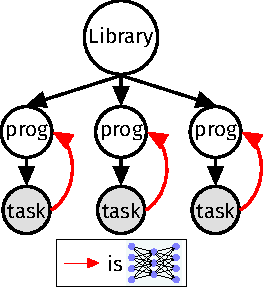
\includegraphics[width = 0.3\textwidth]{cycleGraphicalModel1}}
  \only<2>{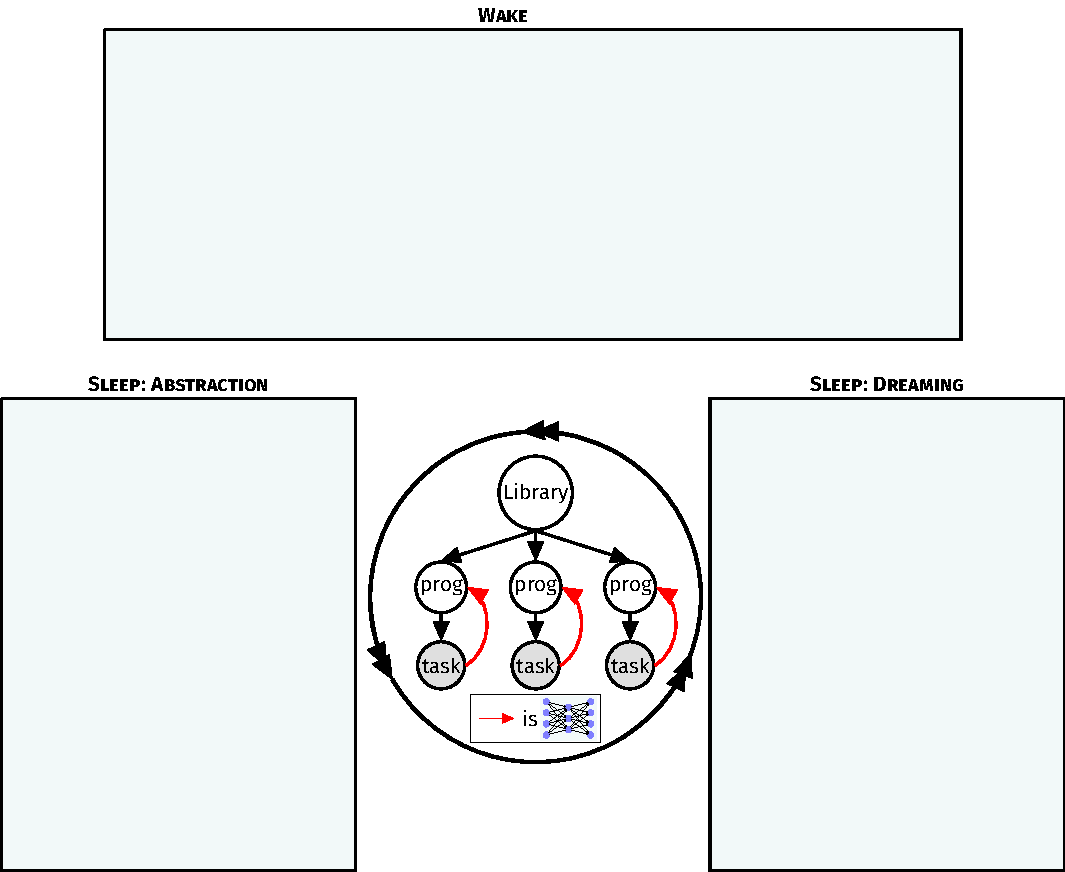
\includegraphics[width = \textwidth]{cycleGraphicalModel2}}
  \only<3>{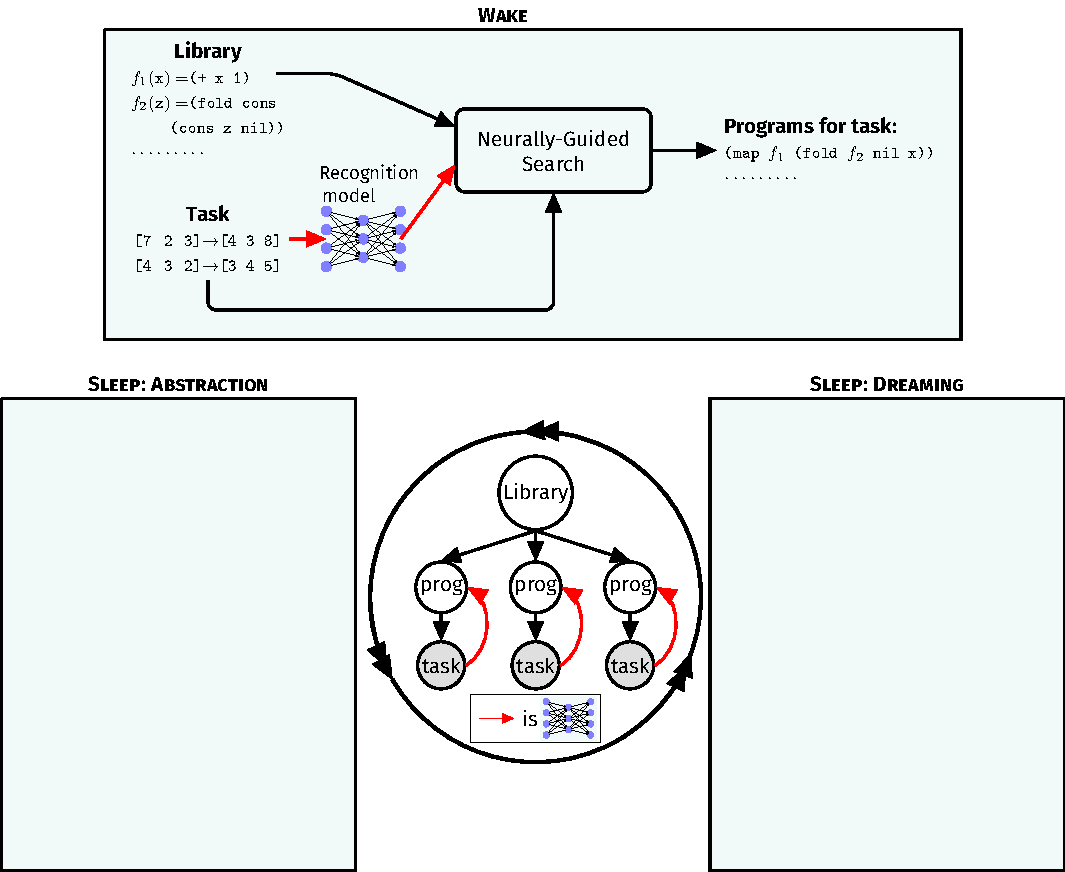
\includegraphics[width = \textwidth]{cycleGraphicalModel3}}
  \only<4>{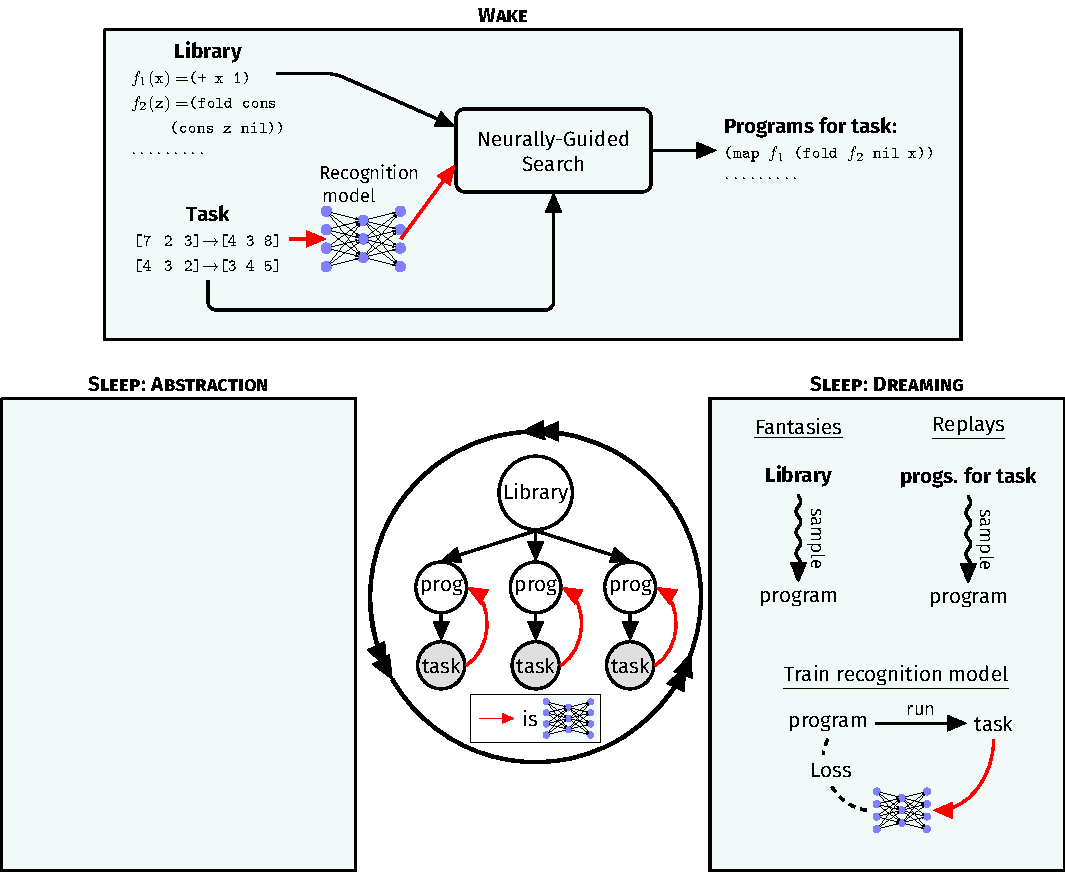
\includegraphics[width = \textwidth]{cycleGraphicalModel4}}
  \only<5>{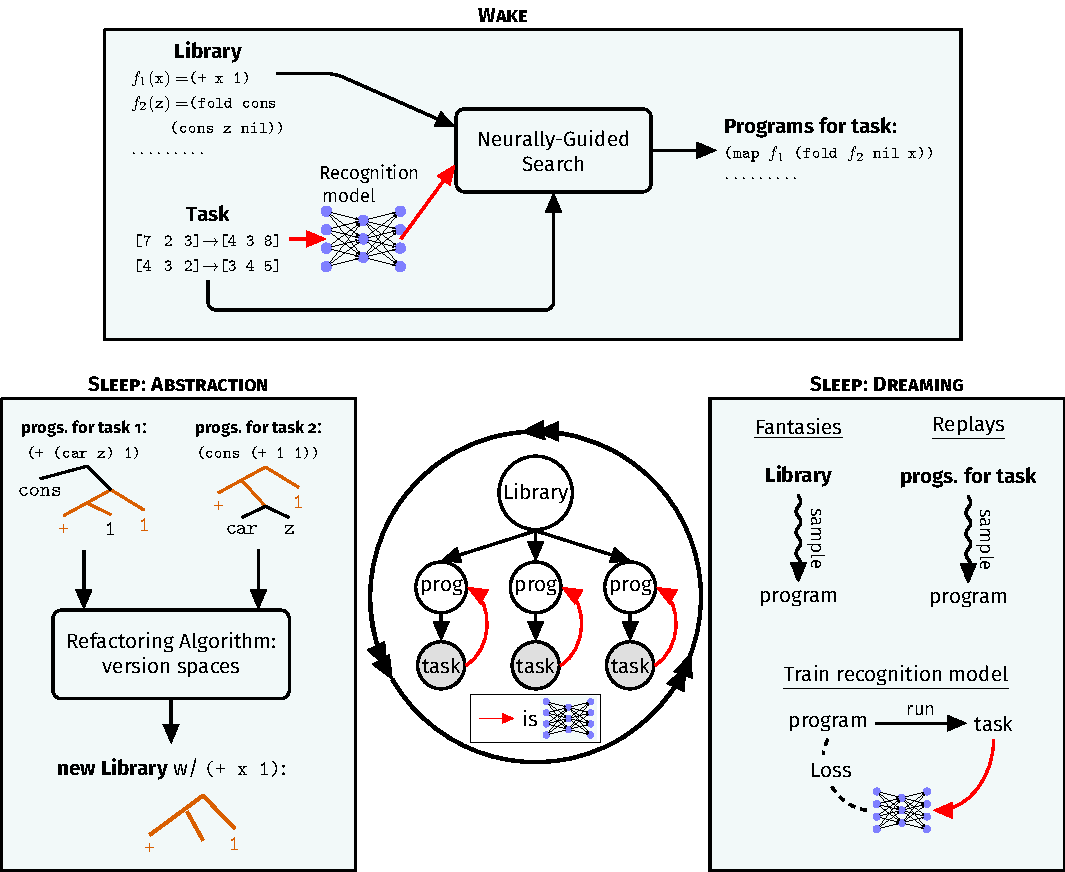
\includegraphics[width = \textwidth]{cycleGraphicalModel5}}
\end{frame}

\begin{frame}{Abstraction Sleep: Growing the library via refactoring}
  \centering
    \Wider[0em]{\begin{tikzpicture}[every node/.style={inner sep=1,outer sep=0,rounded corners,thick, scale=0.7}]
  \footnotesize
  \node(p1)[draw,rounded corners,thick] at (-1,0) {
    \begin{tabular}{l}
      \texttt{(Y ($\lambda$ (r l) (if (nil? l) nil}\\
      \texttt{ (cons (+ (car l) (car l))}\\
      \phantom{\texttt{(cons }}\texttt{ (r (cdr l))))))}
    \end{tabular}
  };
  
  \node(p2)[draw] at ([xshift=4cm]p1.east) {
    \begin{tabular}{l}
      \texttt{(Y ($\lambda$ (r l) (if (nil? l) nil}\\
      \texttt{ (cons (- (car l) 1)}\\
      \phantom{\texttt{(cons }}\texttt{ (r (cdr l))))))}
    \end{tabular}
    
  };

    \node(t1)[draw] at ([yshift=1cm]p1.north) {\begin{tabular}{ll}
      \textbf{Task}:&\texttt{(1 2 3)$\to$(2 4 6)}\\
      &\texttt{(4 3 4)$\to$(8 6 8)}
  \end{tabular}};
  \draw [->] (t1.south)  --(p1.north) node[fill=white,midway] {Wake: program search};
  \node(t2)[draw] at ([yshift=1cm]p2.north) {\begin{tabular}{ll}
      \textbf{Task}:&\texttt{(1 2 3)$\to$(0 1 2)}\\
      &\texttt{(4 3 4)$\to$(3 2 3)}
  \end{tabular}};
  \draw [->] (t2.south)  --(p2.north) node[fill=white,midway] {Wake: program search};

  
  \pause
  \node(r1)[draw,inner sep=0,outer sep=0] at ([yshift=-2cm]p1.south) {
    \begin{tabular}{l}
      \texttt{(}\orange{\texttt{($\lambda$ (f) (Y ($\lambda$ (r l) (if (nil? l)}}\\
      \phantom{(($\lambda$ (f) (Y ($\lambda$ (r l)}\orange{\texttt{nil}}\\
      \phantom{(($\lambda$ (f) (Y ($\lambda$ (r l)}\orange{\texttt{(cons (f (car l))}}\\
      \phantom{(($\lambda$ (f) (Y ($\lambda$ (r l)}\orange{\texttt{ (r (cdr l)))))))}}\\
      \texttt{ ($\lambda$ (z) (+ z z)))}
    \end{tabular}
  };

  \node(r2)[draw] at ([yshift=-2cm]p2.south) {
    \begin{tabular}{l}
      \texttt{(}\orange{\texttt{($\lambda$ (f) (Y ($\lambda$ (r l) (if (nil? l)}}\\
      \phantom{(($\lambda$ (f) (Y ($\lambda$ (r l)}\orange{\texttt{nil}}\\
      \phantom{(($\lambda$ (f) (Y ($\lambda$ (r l)}\orange{\texttt{(cons (f (car l))}}\\
      \phantom{(($\lambda$ (f) (Y ($\lambda$ (r l)}\orange{\texttt{ (r (cdr l)))))))}}\\
      \texttt{ ($\lambda$ (z) (- z 1)))}
    \end{tabular}

  };

  \draw [->] (p1.south)  --(r1.north) node[fill=white,midway,align=center] {refactor\\($10^{14}$ refactorings)};
  \draw [->] (p2.south)  --(r2.north) node[fill=white,midway,align=center] {refactor\\($10^{14}$ refactorings)};



    \node(dummy) at ($(0,1) + (r1.north)!0.5!(r2.north)$) {};
    \node(dummy1) at (r1.west) {\phantom{t}};


    \draw[ultra thick] ($(r1.north west) + (-0.5,1)$) -- ($(r2.north east) + (0.5,1)$)
    -- ($(r2.north east) + (0.5,1) + (0,-5.75)$)
    -- ($(r1.north west) + (-0.5,1) + (0,-5.75)$)
    -- ($(r1.north west) + (-0.5,1)$);
    %  \node(sleepBox)[ultra thick, rounded corners=0, inner sep=25,outer sep=20, draw, fit= (dummy) (r1) (r2) (m) (dummy1) ] {};
    \node at ($(0.0,0.5) + (r1.north)!0.5!(r2.north)$) {{\normalsize\textbf{Sleep: Abstraction}}};

    \pause
    
    \node[draw](m) at ($(0,-2) + (r1.south)!0.5!(r2.south)$) {
      \begin{tabular}{lr}
        &\\
        \code{(}\fbox{\textsc{map}}\code{ ($\lambda$ (z) (+ z z)))}&
        \code{(}\fbox{\textsc{map}}\code{ ($\lambda$ (z) (- z 1)))}\\&\\
        \multicolumn{2}{l}{\fbox{\textsc{map}} = \orange{\texttt{($\lambda$ (f) (Y ($\lambda$ (r l) (if (nil? l) nil}}}\\
        \multicolumn{2}{l}{\phantom{\texttt{\emph{map}} = \texttt{($\lambda$ (f) (Y ($\lambda$ (r l) (if }}\orange{\texttt{(cons (f (car l))}}}\\
        \multicolumn{2}{l}{\phantom{\texttt{\emph{map}} = \texttt{($\lambda$ (f) (Y ($\lambda$ (r l) (if }}\orange{\texttt{(r (cdr l))))))}}}
      \end{tabular}      
    };
    \draw [->](r1.south)--($(-1.75,-0.3) + (m.north)$);
    \draw [->](r2.south)--($(1.75,-0.3) + (m.north)$);
    \node[fill=white] at ([yshift=0.4cm]m.north) {\textbf{Compress (MDL/Bayes objective)}};

    \end{tikzpicture}}
\end{frame}

\begin{frame}{Version space algebra for refactoring}
  \begin{tabular}{lr}
    \begin{tabular}{l}
      Expr\phantom{$\vert$}$\to $ var\\
      \phantom{Exprtt}$\vert$ $\lambda $var.Expr\\
      \phantom{Exprtt}$\vert$ (Expr Expr)\\
      \phantom{Exprtt}$\vert$ primitive\\
      \phantom{VStt$\vert$ VS$\uplus$VS}    \\
      \phantom{VStt$\vert$ $\Lambda$}    \\
      \phantom{VStt$\vert$ $\varnothing$    }

    \end{tabular}&
    \visible<2->{\begin{tabular}{lr}
      VS\phantom{$\vert$}$\to $ var\\
      \phantom{VStt}$\vert$ $\lambda $var.VS\\
      \phantom{VStt}$\vert$ (VS VS)\\
      \phantom{VStt}$\vert$ primitive    \\
      \phantom{VStt}$\vert$ VS$\uplus$VS&\emph{nondeterministic choice}    \\
      \phantom{VStt}$\vert$ $\Lambda$&\emph{choose any expression}    \\
      \phantom{VStt}$\vert$ $\varnothing$    &\emph{choose no expression}
    \end{tabular}}
  \end{tabular}

  
  \visible<3>{what version spaces mean:\begin{align*}
      \denotation{\text{var}}& = \left\{\text{var} \right\}&
      \denotation{v_1 \uplus v_2}& = \left\{e : v\in \left\{v_1,v_2 \right\},\;e\in \denotation{v} \right\}\\
      \denotation{\lambda x. v}& = \left\{\lambda x. e : e\in \denotation{v} \right\}&    
      \denotation{(v_1\; v_2)}& = \left\{(e_1\;e_2) : e_1\in \denotation{v_1},\;e_2\in \denotation{v_2} \right\}\\
      \denotation{\varnothing}& = \varnothing&
      \denotation{\Lambda}& = \Lambda
  \end{align*}}

\end{frame}

\begin{frame}{Using version spaces}
  \begin{tabular}{lr}
    \multicolumn{2}{l}{VS\phantom{$\vert$}$\to $ var\phantom{t}$\vert$ $\lambda $var.VS\phantom{t}$\vert$ (VS VS)\phantom{t}$\vert$ primitive}    \\
    \phantom{VStt}$\vert$ VS$\uplus$VS&\emph{nondeterministic choice}    \\
    \phantom{VStt}$\vert$ $\Lambda$&\emph{choose any expression}    \\
    \phantom{VStt}$\vert$ $\varnothing$    &\emph{choose no expression}
  \end{tabular}

  \vfill
  
\only<2>{exploit the fact that $e\in \denotation{v}$ can be efficiently computed:  
  \begin{align*}
  \textsc{refactor}(v|\text{Lib}) &= \begin{cases}
    e\text{, if $e\in \text{Lib}$ and $e\in \denotation{v}$}\\
    \textsc{refactor}'(v|\text{Lib})\text{, otherwise.}
  \end{cases}
\end{align*}
\begin{align*}
  \textsc{refactor}'(v|\text{Lib})& = v\text{, if $v$ is a primitive or variable}\\
  \textsc{refactor}'(\lambda x.b|\text{Lib}) &= \lambda x. \textsc{refactor}(b|\text{Lib})\\
  \textsc{refactor}'(v_1\;v_2|\text{Lib}) &= (\textsc{refactor}(v_1|\text{Lib})\phantom{t}\textsc{refactor}(v_2|\text{Lib}))\\
%  \textsc{refactor}'(v_1 \uplus v_2|\text{Lib}) &= \argmin_{e\in \left\{\textsc{refactor}(v|\text{Lib})\;:\;v\in V \right\}}\text{size}(e|\text{Lib})
  \end{align*}}

\only<3->{%% invert $\beta$-reduction via new $I\beta$ operator
  \centering

  \begin{tikzpicture}[every node/.style={inner sep=1,outer sep=0,rounded corners,thick}]
    \node[draw, rounded corners](u1) at (0,0) {union, $\uplus$};
    \node[draw, rounded corners](u2) at ($(0,-1) + (u1.south)$) {\code{(}$\uplus$\code{ 1)}}; \draw (u1.south) -- (u2.north);
    \node[draw, rounded corners](u21) at ($(-1.3,-1) + (u2.south)$) {\code{(($\lambda$ (x) (x 1)) +)}}; \draw ([xshift=-0.2cm]u2.south) -- (u21.north);
    \node[draw, rounded corners](u22) at ($(2.3,-1) + (u2.south)$) {\code{(($\lambda$ (x) (+ x)) 1)}};  \draw ([xshift=-0.2cm]u2.south) -- (u22.north);

    \node[draw, rounded corners](u11) at ($(-1.75,-1) + (u1.south)$) {\code{(+ 1 1)}}; \draw (u1.south) -- (u11.north);
    \node[draw, rounded corners](u12) at ($(2.75,-1) + (u1.south)$) {\code{(($\lambda$ (x) (x 1 1)) +)}}; \draw (u1.south) -- (u12.north);

    \node(vs) at ($(u21.west)!0.5!(u12.east) + (0,-1.25)$) {$\underbrace{\hspace{8cm}}_{\text{\normalsize Subset of version space}}$};

    \node[anchor=north](p) at ($(0,2.5) + (u1)$) {\normalsize Program: \texttt{(+ 1 1)}};
    \draw[ultra thick,->] ($(0,-0.1) + (p.south)$) --node[sloped, above, inner sep=5]{$I\beta$} ($(0,0.1) + (u1.north)$);  
\end{tikzpicture}
}

\only<4>{
  \messageOverlay{\textbf{completeness:} $I\beta$ gets all the refactorings\\
    let $v_2 = I\beta(v_1)$ and $e_1\in \denotation{v_1}$. for any $e_2\reduce e_1$ then $e_2\in \denotation{v_2}$\\\\
    \textbf{consistency:} $I\beta$ only gets valid refactorings\\
    let $v_2 = I\beta(v_1)$ and $e_2\in \denotation{v_2}$. then there is a $e_1\in \denotation{v_1}$ where $e_2\reduce e_1$
  }
  }

\end{frame}






%% \begin{frame}{DreamCoder --- Sleep-R (\textbf{Experience Replay})}
%%   \only<1>{
%%     \includegraphics[width=11cm]{ecFigures/teachDC/.inkslides-sleep-r-1/slide-4.pdf}
%%   }
%% \end{frame}
%% \begin{frame}{DreamCoder --- Sleep-R (\textbf{Dreaming})}
%%   \only<1>{
%%     \includegraphics[width=11cm]{ecFigures/teachDC/.inkslides-sleep-r-2/slide-4.pdf}
%%   }
%% \end{frame}
 

%% \begin{frame}{List functions --- \small{Created \& investigated by Lucas
%%   Morales}}


%%   \vspace{1cm}
  
%%   \begin{figure}[b]\centering
%% \vspace{-0.5cm}  \begin{tabular}{lll}
%%     \toprule
%%     Name & Input & Output \\\midrule
%%     repeat-3 & [7\, 0] & [7\, 0\, 7\, 0\, 7\, 0] \\
%%     drop-3 & [0\, 3\, 8\, 6\, 4] & [6\, 4] \\
%%     rotate-2 & [8\, 14\, 1\, 9] & [1\, 9\, 8\, 14] \\
%%     count-head-in-tail & [1\, 2\, 1\, 1\, 3] & 2 \\
%%     keep-div-5 & [5\, 9\, 14\, 6\, 3\, 0] & [5\, 0] \\
%%     product & [7\, 1\, 6\, 2] & 84 \\
%%     \bottomrule
%%   \end{tabular}
%%   %\captionof{table}{Some tasks in our list function domain.}\label{listExamples}\vspace{-0.5cm}
%% \end{figure}

%%   Discovers 38 concepts, including `filter'. %With different tasks will also learn `map', `fold', `unfold', etc. starting with 1950's Lispthe
  
%% \begin{picture}(50,70) \put(250,0){\hbox{\includegraphics[width = 3cm]{ecFigures/Lucas}}} \end{picture} 
%% \end{frame}


%% \begin{frame}{Text editing}
%%   In the style of FlashFill (Gulwani 2012)

%%   \centering  \includegraphics[width = 5cm]{textColumn.png}

%% \vspace{-0.5cm}  SyGuS problems: solves 3\% before learning, vs 75\% after learning. Best prior work: 80\%

%% \end{frame}$

%% \begin{frame}{List functions \& Text editing: Learning curves on hold out tasks}

%%   \begin{center}
%%     \includegraphics[width = 5cm]{ecFigures/listLearningCurve.eps}
%% \hfill    \includegraphics[width = 5cm]{ecFigures/textLearningCurve.eps} 
%%     \end{center}

%% Learning curves for DreamCoder both with (\orange{in orange}) and without
%%     (\teal{in teal}) the recognition model. Solid lines: \% holdout testing tasks solved w/ 10m timeout. Dashed lines: Average solve time, averaged only over tasks that are solved.


%% \end{frame}


%% \begin{frame}{Learned text processing DSL}
%%   \only<1>{  \includegraphics[width = \textwidth]{ecFigures/textPrimitives.pdf}}
%%   \only<2>{  \includegraphics[width = \textwidth]{ecFigures/textPrimitives.png}}

%% \end{frame}

%% \begin{frame}{Learning the fundamentals of programming}
%%   \includegraphics[width = \textwidth]{ecFigures/McCarthy.png}

%% \centering  McCarthy 1959 Lisp  $\longrightarrow$ Modern functional programming
  
%%   22 tasks. 64 CPUs. 93 hours.

%%   \end{frame}

%% \begin{frame}{Symbolic regression from visual input}
%% \centering\includegraphics[width = 5cm]{symbolicRegression.png}
%% \end{frame}

\begin{frame}{DreamCoder Domains}
  \only<1>{\includegraphics[width = \textwidth]{statement/taskbar2.png}}
  \only<2>{\includegraphics[width = \textwidth]{statement/taskbar3.png}}
\end{frame}

\begin{frame}{LOGO Graphics}
  30 out of 160 tasks
  \includegraphics[width = \textwidth]{dc/logoTasks30.png}
\end{frame}

\begin{frame}{LOGO Graphics -- learning interpretable library of concepts}
  \Wider[5em]{
    \includegraphics[width = \textwidth]{dc/logo_kathy.png}
  }

  \only<2>{
  \messageOverlay{
    \begin{tabular}{rl}
    circle$(r)$
    &\raisebox{-.5\height}{\includegraphics[width = 0.3\textwidth]{dc/logo_primitives/circle_negative.png}}\\
    polygon$(n,\ell)$
    &\raisebox{-.5\height}{\includegraphics[width = 0.3\textwidth]{dc/logo_primitives/polygon_negative.png}}
  \end{tabular}
  }}
  \only<3>{
    \messageOverlay{\begin{tabular}{c}
    radial symmetry$(n,\text{body})$\\
    \includegraphics[width = 0.35\textwidth]{dc/rotationalmontage_negative.png}
  \end{tabular}}
    }
\end{frame}

\begin{frame}{what does DreamCoder dream of?}
  \Wider[5em]{
    \only<1>{\begin{tabular}{lll}
    before learning&&after learning\\
    \includegraphics[height=3cm]{dc/dreams/beforeLearning25September11}&&
    \includegraphics[height=3cm]{dc/dreams/cherry_picked/montageSeptember14}    
    \end{tabular}}
    \only<2>{\begin{tabular}{lll}
        before learning&&after learning\\
        \includegraphics[width = 0.4\textwidth]{dc/dreams/appendixlogoinitial.png}&&
        \includegraphics[width = 0.4\textwidth]{dc/dreams/appendixlogofinal.png}
        \end{tabular}}
    }

\end{frame}

\begin{frame}{Planning to build towers}
  \Wider[5.5em]{
    \footnotesize
    \begin{tabular}{l}
      {example tasks (112 total)}\\
      \includegraphics[clip, trim = 0 0cm 0 2.9cm,width = 0.9\textwidth]{dc/tower_montage_21_negative.png}\\\\

    \end{tabular}
    \pause
    \begin{tabular}{l}
      {learned library routines ($\approx $ 20 total)}\\
      \begin{tabular}[t]{rlrl}
        arch$(h)$&%\begin{tabular}{l}
        \raisebox{-.1\height}{\includegraphics[width = 0.25\textwidth]{dc/tower/tower_dsl_towerArch.png}}&
        %\end{tabular}&
        pyramid$(h)$&
        \raisebox{-.1\height}{\includegraphics[width = 0.25\textwidth]{dc/tower/tower_dsl_pyramid.png}}
        \\
        wall$(w,h)$&
        \raisebox{-.3\height}{\includegraphics[width = 0.25\textwidth]{dc/tower/tower_dsl_bricks.png}}
        &%\\\\
        %% stairs$(h)$&\begin{tabular}{l}
        %%   \includegraphics[width = 0.25\textwidth]{dc/tower/tower_dsl_staircase.png}
        %% \end{tabular}\\\\
        \phantom{bbb}bridge$(w,h)$&
        \raisebox{-.3\height}{\includegraphics[width = 0.25\textwidth]{dc/tower/tower_dsl_bridge.png}}
        %\\\\\\
      \end{tabular}\\\\

  \end{tabular}}

  \pause

  \messageOverlay{
    \begin{tabular}{ll}
          \textbf{dreams before learning}&\textbf{dreams after learning}\\
          \begin{tabular}{c}
            \includegraphics[clip,trim = 0 4.5cm 0 0cm,width = 0.4\textwidth]{dc/tower/dreams/cherry_montage_initial_20.png}
          \end{tabular}\phantom{testing}&
          \begin{tabular}{c}
            \includegraphics[clip,trim = 0 4.5cm 0 0cm,width = 0.4\textwidth]{dc/tower/dreams/cherry_montage_final.png}
            \end{tabular}
          \\\\
      \end{tabular}
  }
  
\end{frame}

\begin{frame}{synergy between dreaming and library learning}
    \begin{tabular}{ll}
      %    \textbf{A}\\
      \only<1>{\includegraphics[height = 2cm]{../dreamcoder/figures/learningCurves/revision/text_hits_average_pretty_small_yl_stage1.png}}
      \only<2>{\includegraphics[height = 2cm]{../dreamcoder/figures/learningCurves/revision/text_hits_average_pretty_small_yl_stage2.png}}
      \only<3>{\includegraphics[height = 2cm]{../dreamcoder/figures/learningCurves/revision/text_hits_average_pretty_small_yl_stage3.png}}
      \only<4->{\includegraphics[height = 2cm]{../dreamcoder/figures/learningCurves/revision/text_hits_average_pretty_small_yl.png}}
      &
      \phantom{ttt}%
      \only<1>{\includegraphics[height = 2cm]{../dreamcoder/figures/learningCurves/revision/logo_hits_average_pretty_small_stage1.png}}
      \only<2>{\includegraphics[height = 2cm]{../dreamcoder/figures/learningCurves/revision/logo_hits_average_pretty_small_stage2.png}}
      \only<3>{\includegraphics[height = 2cm]{../dreamcoder/figures/learningCurves/revision/logo_hits_average_pretty_small_stage3.png}}
      \only<4->{\includegraphics[height = 2cm]{../dreamcoder/figures/learningCurves/revision/logo_hits_average_pretty_small.png}}\\
      \only<1>{\includegraphics[height = 2cm]{../dreamcoder/figures/learningCurves/revision/list_hard_hits_average_pretty_small_yl_stage1.png}}
      \only<2>{\includegraphics[height = 2cm]{../dreamcoder/figures/learningCurves/revision/list_hard_hits_average_pretty_small_yl_stage2.png}}
      \only<3>{\includegraphics[height = 2cm]{../dreamcoder/figures/learningCurves/revision/list_hard_hits_average_pretty_small_yl_stage3.png}}
      \only<4->{\includegraphics[height = 2cm]{../dreamcoder/figures/learningCurves/revision/list_hard_hits_average_pretty_small_yl.png}}&
      \phantom{ttt}%
      \only<1>{\includegraphics[height = 2cm]{../dreamcoder/figures/learningCurves/revision/rational_hits_average_pretty_small_stage1.png}}
      \only<2>{\includegraphics[height = 2cm]{../dreamcoder/figures/learningCurves/revision/rational_hits_average_pretty_small_stage2.png}}
      \only<3>{\includegraphics[height = 2cm]{../dreamcoder/figures/learningCurves/revision/rational_hits_average_pretty_small_stage3.png}}
      \only<4->{\includegraphics[height = 2cm]{../dreamcoder/figures/learningCurves/revision/rational_hits_average_pretty_small.png}}\\
      \only<1>{\includegraphics[height = 2.29cm]{../dreamcoder/figures/learningCurves/revision/tower_hits_ws_average_pretty_small_yl_stage1.png}}
      \only<2>{\includegraphics[height = 2.29cm]{../dreamcoder/figures/learningCurves/revision/tower_hits_ws_average_pretty_small_yl_stage2.png}}
      \only<3>{\includegraphics[height = 2.29cm]{../dreamcoder/figures/learningCurves/revision/tower_hits_ws_average_pretty_small_yl_stage3.png}}
      \only<4->{\includegraphics[height = 2.29cm]{../dreamcoder/figures/learningCurves/revision/tower_hits_ws_average_pretty_small_yl.png}}&
      \phantom{tt.}%
      \only<1>{\includegraphics[height = 2.29cm]{../dreamcoder/figures/learningCurves/revision/regex_marginal_test_unigram_gen_ws_stage1.png}}
      \only<2>{\includegraphics[height = 2.29cm]{../dreamcoder/figures/learningCurves/revision/regex_marginal_test_unigram_gen_ws_stage2.png}}
      \only<3>{\includegraphics[height = 2.29cm]{../dreamcoder/figures/learningCurves/revision/regex_marginal_test_unigram_gen_ws_stage3.png}}
      \only<4->{\includegraphics[height = 2.29cm]{../dreamcoder/figures/learningCurves/revision/regex_marginal_test_unigram_gen_ws.png}}%
%    \includegraphics[height = 2.29cm]{../dreamcoder/figures/learningCurves/revision/regex_marginal_test_unigram_gen_ws.png}%
    \phantom{tt}\includegraphics[width = 2.5cm]{../dreamcoder/figures/learningCurves/revision/curveLegend.png}\hspace{-3cm}
    %    \includegraphics[width = 0.25\textwidth]{../dreamcoder/figures/learningCurves/revision/depthVersusAccuracy_revision_MAX.png}
    \end{tabular}


      %% }
      %% }

\end{frame}

\begin{frame}{synergy between dreaming and library learning}
  \begin{tikzpicture}[scale=1.5]
    {
    \begin{scope}[shift = {(1,-1)}]
    \node[align = center](synthesis) at (6,4) {Problem-solving};
    \node[align = center](Library) at (3,1) {Library};
    \node[align = center](recognitionModel) at (9,1) {Recognition \\model};

    \draw [->,thick] (synthesis.-120) to[out = -150,in = 60] node[below,rotate = 45,align = center]{{\footnotesize Trains}\\{\footnotesize (Abstraction)}} (Library.30);
    \draw [->,thick] (synthesis.-60) to[out = -30,in = 120] node[below,rotate=-45,align = center]{{\footnotesize Trains}\\{\footnotesize (Dreaming)}} (recognitionModel.150);
    \draw [->,thick] (Library.east) to[out = -30,in = 210] node[above, align = center]{{\footnotesize Trains}\\{\footnotesize (Dreaming)}} (recognitionModel.west);

    \draw [->,thick,dashed] (Library.north) to[out = 90,in = 180] node[fill=white,inner sep=0pt,align = center]{  \footnotesize{Inductive bias}\\\footnotesize{Hypothesis space}\\\footnotesize{(Wake)}} (synthesis.west);
    \draw [->,thick,dashed] (recognitionModel.north) to[out = 90,in = 0] node[fill=white,inner sep=0pt,align = center]{{\footnotesize Makes tractable}\\{\footnotesize (Wake)}} (synthesis.east);
  \end{scope}}
    \end{tikzpicture}

\end{frame}

\begin{frame}{Evidence for dreaming bootstrapping better libraries}
    \begin{tabular}{rr}
%        \multicolumn{1}{l}{\textbf{B}}\\
    \includegraphics[height = 0.3\textwidth]{../dreamcoder/figures/learningCurves/revision/depthVersusAccuracy_revision_MEAN.png}&
    \includegraphics[height = 0.3\textwidth]{../dreamcoder/figures/learningCurves/revision/depthVersusAccuracy_revision_SIZE.png} \\\\
\multicolumn{2}{c}{    \includegraphics[height = 1cm]{../dreamcoder/figures/learningCurves/revision/scatterLegend.png}}
    \end{tabular}
    Dark$\to $Light: Early in learning$\to $Later in learning

  \end{frame}




\end{document}
